%-----------------------------------LICENSE------------------------------------%
%   This file is part of tikz_figures.                                         %
%                                                                              %
%   tikz_figures is free software: you can redistribute it and/or              %
%   modify it it under the terms of the GNU General Public License as          %
%   published by the Free Software Foundation, either version 3 of the         %
%   License, or (at your option) any later version.                            %
%                                                                              %
%   tikz_figures is distributed in the hope that it will be useful,            %
%   but WITHOUT ANY WARRANTY; without even the implied warranty of             %
%   MERCHANTABILITY or FITNESS FOR A PARTICULAR PURPOSE.  See the              %
%   GNU General Public License for more details.                               %
%                                                                              %
%   You should have received a copy of the GNU General Public License along    %
%   with tikz_figures.  If not, see <https://www.gnu.org/licenses/>.           %
%------------------------------------------------------------------------------%

% Use the standalone class for displaying the tikz image on a small PDF.
\documentclass[crop, tikz]{standalone}

% Import the tikz package to use for the drawing.
\usepackage{tikz}

% Tikz packages used.
\usetikzlibrary{arrows.meta}

% Begin the document.
\begin{document}

    % Begin the drawing.
    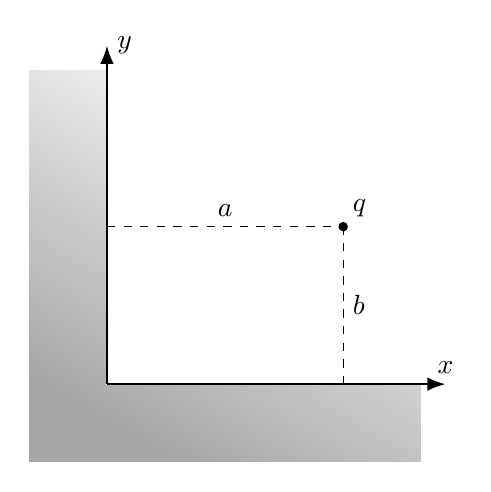
\begin{tikzpicture}[> = Latex]

        % Positions for all of the points.
        \coordinate (O) at (0.0, 0.0);
        \coordinate (A) at (0.0, 4.0);
        \coordinate (B) at (-1.0, 4.0);
        \coordinate (C) at (-1.0, -1.0);
        \coordinate (D) at (4.0, -1.0);
        \coordinate (E) at (4.0, 0.0);
        \coordinate (Q) at (3.0, 2.0);
        \coordinate (QX) at (3.0, 0.0);
        \coordinate (QY) at (0.0, 2.0);
        \coordinate (X) at (4.3, 0.0);
        \coordinate (Y) at (0.0, 4.3);

        % Draw the conducting region and shade it.
        \draw[%
            fill,
            bottom color = gray!70!white,
            top color = white,
            draw = white,
            shading angle = 330
        ] (A) to (B) to (C)  to (D) to (E) to (O) to cycle;

        % Draw and label the coordinate axes.
        \draw[->, thick] (O) to (X) node[above] {$x$};
        \draw[->, thick] (O) to (Y) node[right] {$y$};

        % The point charge q and projections on to the coordinate axes.
        \draw[fill = black] (Q) circle (1.5pt);
        \draw[dashed] (QX) to node[right] {$b$} (Q);
        \draw[dashed] (QY) to node[above] {$a$} (Q);
        \node at (Q) [above right] {$q$};
    \end{tikzpicture}
\end{document}
